%% Copernicus Publications Manuscript Preparation Template for LaTeX Submissions
%% ---------------------------------
%% This template should be used for copernicus.cls
%% The class file and some style files are bundled in the Copernicus Latex Package, which can be downloaded from the different journal webpages.
%% For further assistance please contact Copernicus Publications at: production@copernicus.org
%% http://publications.copernicus.org/for_authors/manuscript_preparation.html
%% Please use the following documentclass and journal abbreviations for discussion papers and final revised papers.

\documentclass[acp, manuscript]{copernicus} % single column manuscript: used for both discussion and submission

\begin{document}
\title{Isoprene emissions over Australia}

% \Author[affil]{given_name}{surname}
\Author[1]{Jesse W.}{Greenslade}
\Author[1,2]{Jenny A.}{Fisher}

\affil[1]{Centre for Atmospheric Chemistry, School of Chemistry, University of Wollongong, Australia}
\affil[2]{School of Earth \& Environmental Sciences, University of Wollongong, Australia}

\runningtitle{Australian isorene emissions}
\runningauthor{Greenslade et al.}
\correspondence{Jesse Greenslade (jwg366@uowmail.edu.au)}

%% These dates will be inserted by Copernicus Publications during the typesetting process.
\firstpage{1}
\maketitle

\begin{abstract}
  
\end{abstract}

% Section 1 -- INTRO
\introduction  %% \introduction[modified heading if necessary]

  Emissions of isoprene may be overestimated in Australia.
  One of the most popular emissions inventories for biogenic isoprene, the Model of Emissions of Gases and Aerosols from Nature (MEGAN) is poorly calibrated for Australian conditions.
  \cite{Muller2008} compared MEGANv2 against emissions calculated using top down estimates from the GOME2 satellite measurements of formaldehyde.
  \cite{Stavrakou2015} showed that this overestimate may be a factor of 2-3 in January.
  \cite{Sindelarova2014} show how 50\% of the isoprene emissions could be reduced by accounting for lower soil moisture.
  \cite{Emmerson2016} discuss the suitability of MEGAN's isoprene and monoterpene emission factors over southeast Australia, and suggest ...TODO:

  % AIMs paragraph
  Here we introduce how uncertain isoprene emissions are over Australia, and discuss literature which shows how the estimates may be too high.
  Section \ref{sec:MethodsAndData} describes the methods, models, and campaign data we use to determine and analyse isoprene emissions.
  

\section{Methods and data}
  \label{sec:MethodsAndData}
  
  \subsection{GEOS-Chem simulation}
    \label{sec:GEOSChemSimulation}
    The GEOS-Chem global atmospheric chemistry model (V10.01) simulates and records up to 66 chemical species (tracers) in the standard run, at 2 by 2.5$^{\circ}$ horizontal resolution, with 47 levels up to the top of the atmosphere (TOA at 0.01~hPa). 
    Output for an area averaged over 1200 - 1400 local time can be saved for comparison and recalculation with satellite overpass records.
    GEOS-5 meteorological fields from NASA's ...(TODO: ref and note) are used to drive transport and coupled with the chemical module of GEOS-Chem.
  
  \subsection{Campaigns and datasets}
    \label{sec:Campaigns}
    TODO: these summaries.
    OMI summary
    
    Daintree summary (P. Nelson)
    
    MUMBA summary
  
  \subsection{Recalculation of OMI HCHO}
  
  \subsection{Calculation of Emissions}
    % \label{ch_isop:sec:EmissionCalculation} <- thesis label
    \label{sec:EmissionCalculation}
    
    As is done in \citet{Palmer2003, Millet2006, Bauwens2016}, we assume that HCHO, and Isoprene columns are in a steady state, with no horizontal transport.
    In these circumstances the emissions of precursors are easy to calculate as long as we know the molar HCHO yields (Y$_i$) and effective chemical loss rates (k$_i$):
    \begin{equation}
      \Omega_{HCHO} = \frac{1}{k_{HCHO}}\Sigma_i k_i Y_i \Omega_i = \frac{1}{k_{HCHO}}\Sigma_i Y_i E_i
    \end{equation}
    
    We can infer the local (grid space) isoprene emissions (E$_{isop}$) using effective formaldehyde yield from isoprene ($Y_{isop}$).
    \begin{equation} \label{eqn:isop_yield}
      \Omega_{HCHO} = S \times E_{isop} + B
    \end{equation}
    Where \textit{B} is the background HCHO, and $S = Y_{isop}/k_{HCHO}$ is determined monthly as the regression between $\Omega_{HCHO}$ and E$_{isop}$ on daily saved outputs from GEOS-Chem over Australia using 2 by 2.5$^{\circ}$ horizontal resolution.
    
    % Other method: $k_{HCHO}*\Omega_{HCHO}$, and $k_{isop}*\Omega_{isop}$.
    %For an initial estimate of the effective yield from simulated data: we use $k_{HCHO}$, $k_{i}$, $\Omega_{HCHO}$, and $\Omega_i$ outputs from a standard run of GEOS-Chem - which provides one data point per day.
    This gives us a monthly value for $Y_i$ resolved to our 2$^{\circ}$ by 2.5$^{\circ}$ horizontal resolution, which is entirely based on the model.
    Using our measurements of the biogenic HCHO column ($\hat{\Omega}_{HCHO}$) recalculated from the OMI satellite product, we use this derived yield and the same formula to determine our new top-down emissions estimates.
    Figure \ref{fig:E_isop_vs_hcho_model_sample} shows the modelled isoprene emissions and column HCHO concentrations along with the RMA regression line, sampled from grid boxes over Australia for January 2005.
    Some affects from the low emissions in grid boxes which are largely oceanic can be seen and are handled by TODO: handle these and document here.
    
    Modeled background emissions are ignored as they do not affect the calculation of the modeled slope.
    The OMI background is calculated from the averaged column amounts over the remote pacific (15$^{\circ}$ S to 15$^{\circ}$ N, 175 to 120$^{\circ}$ W)
    However, when calculating the $E_{isop}$ from our modeled slope with OMI HCHO and background, we end up with negative emissions wherever the OMI HCHO column is less than the OMI background (as $E_{isop} = \frac{\Omega_{HCHO} - B}{S}$).
    \begin{figure}[!htbp]
      % Figure from GC_tests.py -> isop_hcho_RMA
      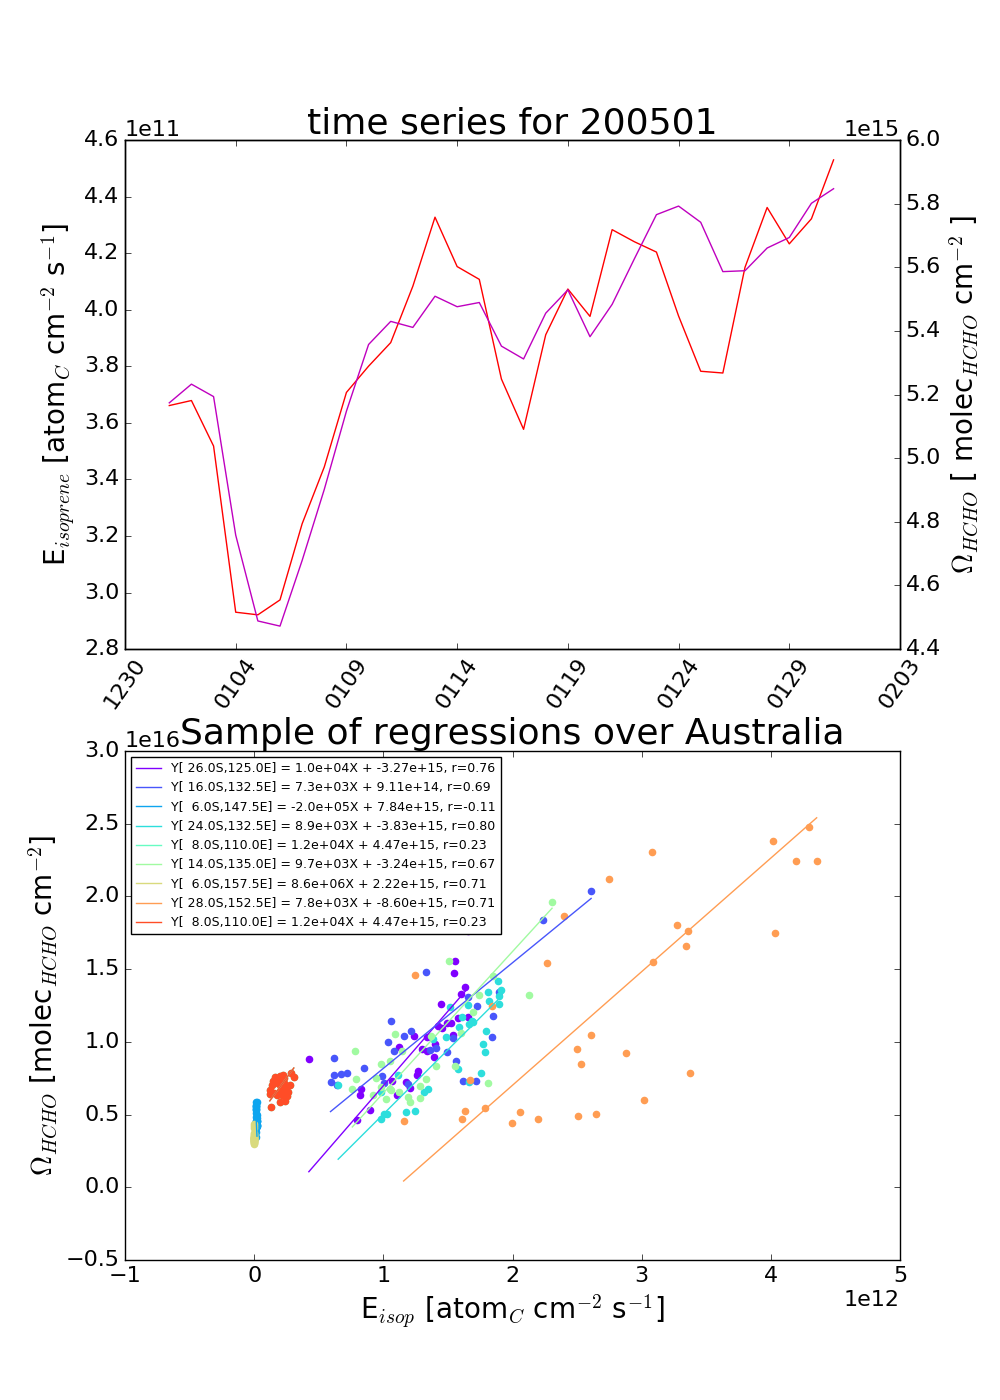
\includegraphics[width=\textwidth]{figures/E_isop_vs_hcho_series_200501.png}
      \caption{%
	Top panel: isoprene emissions for January, 2005, shown in red, coplotted with tropospheric hcho columns, shown in magenta.
	Both series are daily averages over Australia.
	Bottom panel: (RMA) linear regressions from between emissions of isoprene and tropospheric hcho columns, sampled randomly from the 2$^{\circ}$ by 2.5$^{\circ}$ latitude longitude gridboxes over Australia for the month of January (2005).
      }
      \label{fig:E_isop_vs_hcho_model_sample}
    \end{figure}
    
    Using this modelled slope at 2$^{\circ}$ by 2.5$^{\circ}$ and applying it to equation \ref{eqn:isop_yield} with B and $\Omega_{HCHO}$ calculated using OMI satellite measurements provides a new estimate of isoprene emissions.
    Figure TODO: \ref{fig:E_isop_200501} shows the emissions calculated this way along with the Emissions output by GEOS-Chem averaged over January, 2005.
    
    \begin{figure}[!htbp]
      % Figure from Inversion.py -> check_against_MEGAN()
      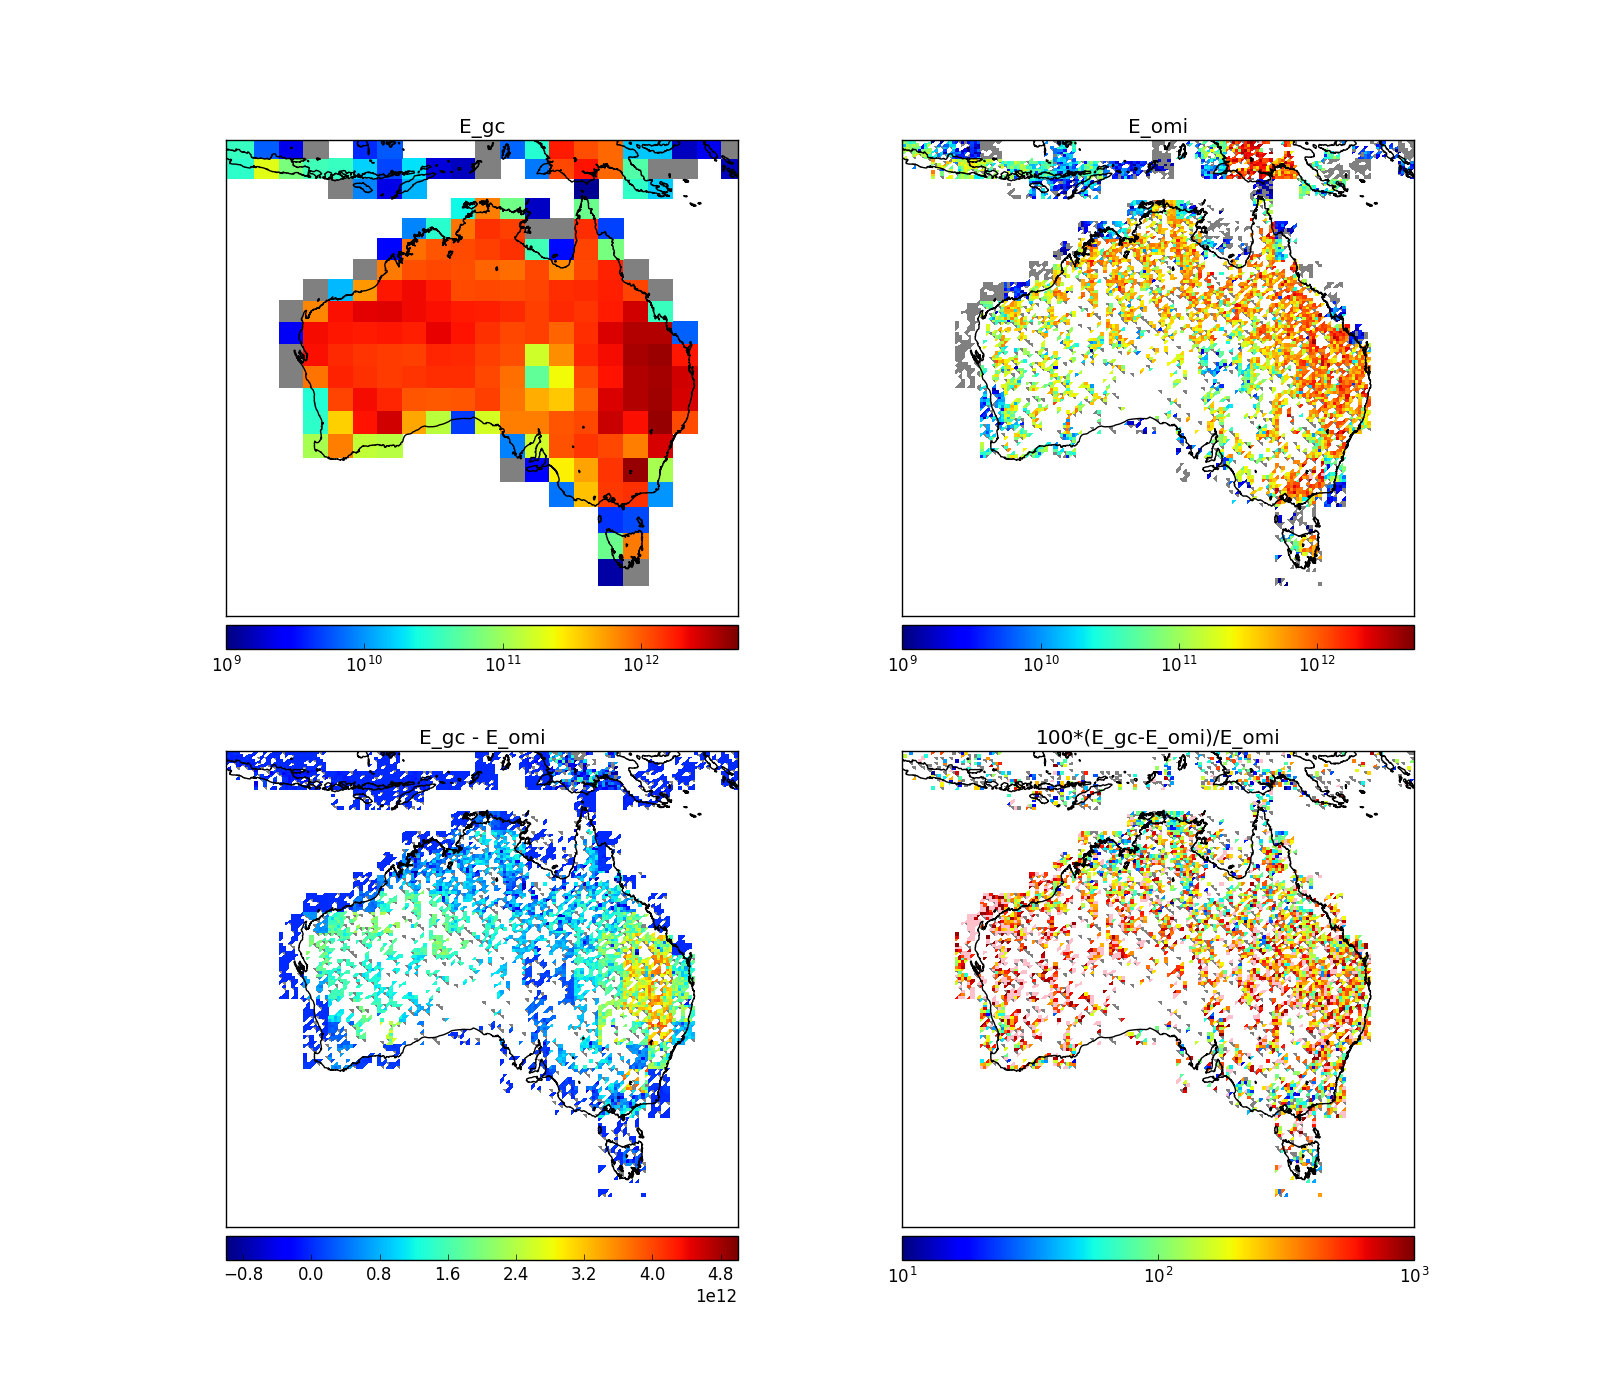
\includegraphics[width=\textwidth]{figures/E_Comparison.png}
      \caption{%
	Top row is isoprene emissions for the month of January, in 2005, from GEOS-Chem and estimated from OMI respectively.
	Bottom row shows the absolute and relative differences between the two.
      }
      \label{fig:E_isop_200501}
    \end{figure}
    
    
\section{Results}
  
  \subsection{Emissions affect on GEOS-Chem}
    We interpolated or something (TODO) the emissions over Australia into the inventories used by GEOS-Chem which reduced the emissions by X\% per year (over Australia).
    The resulting simulation output shows that HCHO was reduced by X\%, although if we boost monoterpenes by X\% where the isoprene emissions were lowered then 
    
  \subsection{Emissions comparisons}
    
    When comparing the GEOS-Chem (which runs MEGAN) emissions to those calculated using our top-down inversion, we see a decrease over TODO: locations and seasons.
    TODO: table or figure showing summary of isoprene emissions changes over the whole of our time domain.
    
    One set of data from the Daintree rainforest in Queensland exists (TODO: summary from P. Nelson).
    Although the data set lies outside our run times, as it was measured in TODO(runtime), we compare against the seasonal average of our GEOS-Chem output for the matching months (TODO: name the months).
    This is done for both GEOS-Chem output and our recalculated isoprene emissions.
    When compared against GEOS-Chem output we see TODO.
    When compared against recalculated emissions we see TODO.
    
    TODO: Figure showing campaign data against model and recalculated emissions over region for averaged months and eventually different resolutions.
    
    
    
\conclusions  %% \conclusions[modified heading if necessary]


\appendix
% \section{}    %% Appendix A
% \subsection{}     %% Appendix A1, A2, etc.

\appendixfigures  %% needs to be added in front of appendix figures in one-column style (\documentclass[acp, manuscript]{copernicus})
\appendixtables   %% needs to be added in front of appendix tables in one-column style (\documentclass[acp, manuscript]{copernicus})

\authorcontribution{}

\competinginterests{The authors declare that they have no conflict of interest.}

%\disclaimer{disclaimer}

% Data availability
%
\textit{Data availability.} All GEOS-Chem model output is available from the authors upon request.

\begin{acknowledgements}
This research is supported by an Australian Government Research Training Program (RTP) Scholarship.
\end{acknowledgements}

%% Since the Copernicus LaTeX package includes the BibTeX style file copernicus.bst,
%% authors experienced with BibTeX only have to include the following two lines:
%%
\bibliographystyle{copernicus}
\bibliography{bibliography/hcho.bib}

\end{document}
